\section{Vehicel Kinematics and Dynamics}
\label{vehicle_kinematics_and_dynamics}

In this section, we will cover kinematic and dynamic modeling of an autonomous car. 
Creating a good vehicle model is essential for model-based control development. 
We'll look at modeling, both the evolution of the kinematics, that is, positions and velocities, and the dynamics or forces and torques of a car and how they connect. 
Later on in the next modules, we will use these vehicle models extensively for controller design. 


In this section, we will study

\begin{itemize}
\item Vehicle kinematics
\item Bicycle model
\item Longitudinal vehicle dynamics
\item Lateral vehicle dynamics
\end{itemize}

\begin{framed}
\theoremstyle{remark}
\begin{remark}{\textbf{Coordinate Transformations}}

Coordinate frames and transformations are explained in the appendix.
\end{remark}
\end{framed}

 
\subsection{Kinematic Modeling}
\label{kinematic_modeling}

So, let's get started. Generally, vehicle motion can be modeled either by considering the geometric constraint that defines its motion or by considering all of the forces and moments acting on a vehicle. 
The first case is known as Kinematic Modeling. Especially at low speeds when the accelerations are not significant, Kinematic Modeling is more than sufficient to capture the motion of a vehicle. When we instead include knowledge of the forces and moments acting on the vehicle, we're performing Dynamic Modeling. 
Dynamic models can do a great job of estimating vehicle motion throughout the vehicles operating range, but are more involved to develop than kinematic models. 

The robot's motion is constrained to move forward because its wheels point in this direction. 
This constraint is called a nonholonomic constraint, which means that it restricts the rate of change of the position of our robot. Mathematically, this can be expressed as follows:

\begin{equation}
\dot{y}\cos(\theta) - \dot{x}\sin(\theta) = 0
\end{equation} 


So, our robot can roll forward and turn while rolling, but cannot move sideways directly. We'll use this constraint to define a kinematic model for our robot. The velocity of the robot is defined by the tangent vector to its path see figure \ref{vehicle_path}. 

\begin{figure}[!htb]
\begin{center}
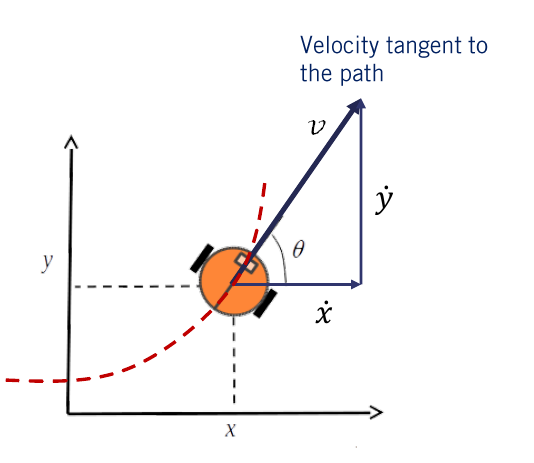
\includegraphics[scale=0.290]{img/kinematics/vehicle_path.jpeg}
\end{center}
\caption{Vehicle velocity.}
\label{vehicle_path}
\end{figure}


Let's define the orientation angle of the robot as $\theta$. Then $\tan(\theta)$ can be written as $dy$ over $dx$. 
The velocity of the robot in the y-direction divided by the velocity of the robot in the x-direction. 
By rearranging the above equation, we can derive an expression for the nonholonomic constraint equation as follows. 
We can then construct a pair of equations for the motion of the robot by combining these equations. 


\begin{equation}
\dot{x} = v \cos(\theta), ~~ \dot{y} = v\sin(\theta)
\end{equation}


We can assume the direct control over the robots rate of change of heading. We've now successfully built a kinematic model for our robot. This model takes as input the forward velocity in rotation rate and represents the robot using a vector of three states, the $x$ and $y$ position of the robot and it's heading. 


\begin{framed}
\theoremstyle{remark}
\begin{remark}{\textbf{State}}

A state is a set of variables often arranged in the form of a vector that fully describe the system at the current time.
\end{remark}
\end{framed}

The input of the model are velocity $v$ and rate of change of orientation $\omega$. 

\begin{figure}[!htb]
\begin{center}
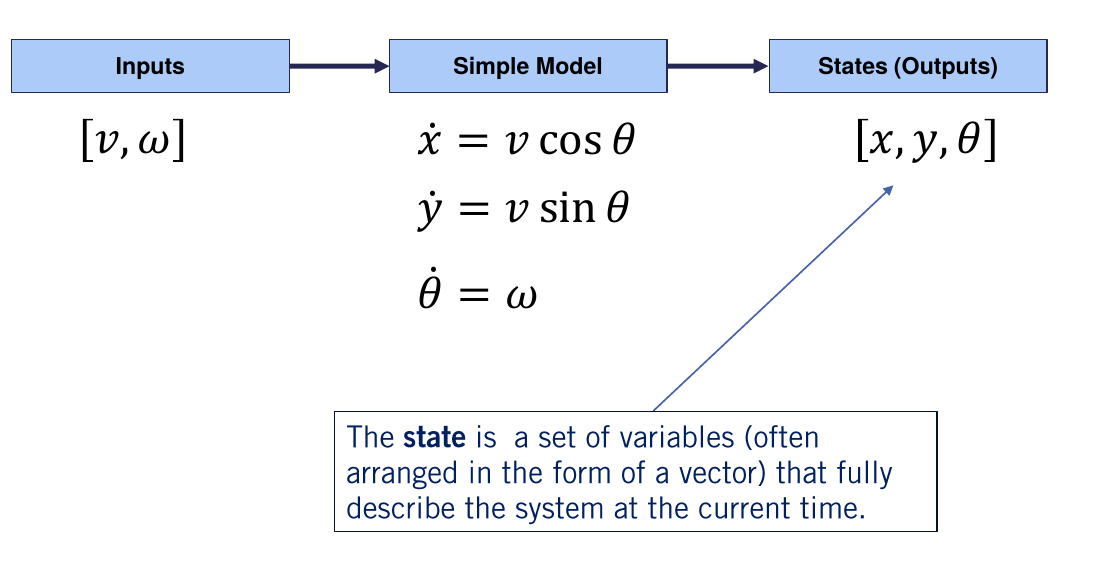
\includegraphics[scale=0.290]{img/kinematics/simple_robot_motion_kinematics.jpeg}
\end{center}
\caption{Simple robot motion kinematics.}
\label{simple_robot_motion_kinematics}
\end{figure}

However, for the actual two-wheel robot, it's also possible we need to directly command wheel velocities as inputs. We'll now look at how to extend our model and relate each wheel rotational velocity to forward velocity, $v$, and rotation rate $\omega$. We'll need a few more variables defined as follows. $P$ is the center of the robot, $L$ is the distance from the center of the robot to each of its wheels, $R$ is the radius of the wheels, $w_1$ and $w_2$ are the left and right wheel angular speeds. 

\begin{figure}[!htb]
\begin{center}
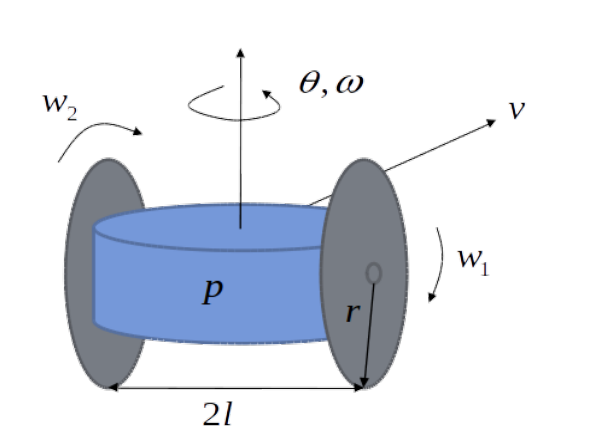
\includegraphics[scale=0.290]{img/kinematics/two_wheels_robot.jpeg}
\end{center}
\caption{Two wheels robot model.}
\label{two_wheels_robot}
\end{figure}


The velocity of the robot at each wheel is the radius of the wheel times its rotational velocity. 

\begin{equation}
 v =r \times w_i
\end{equation}

\begin{figure}[!htb]
\begin{center}
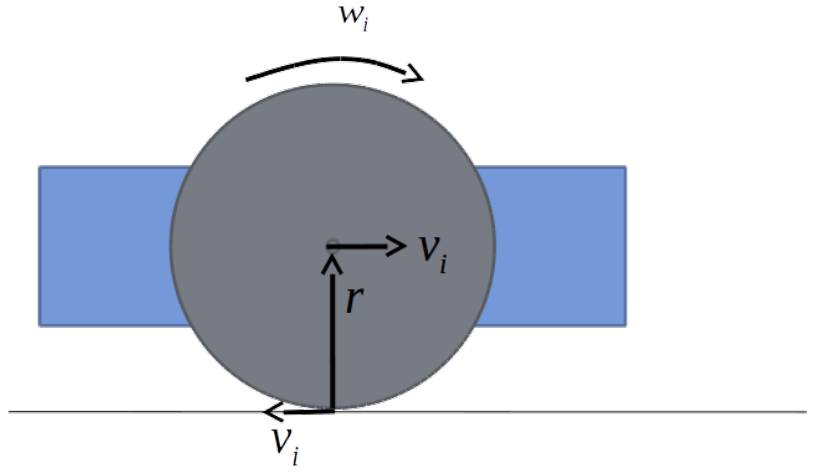
\includegraphics[scale=0.290]{img/kinematics/two_wheels_robot_kinematic_constraint.jpeg}
\end{center}
\caption{Two wheels robot model.}
\label{two_wheels_robot_kinematic_constraint}
\end{figure}

We can do this by assuming no slip between the wheel and the surface. The velocity of the robot can be computed as the average velocity of both wheels as seen from this figure. When the velocities of both wheels are the same, the robot moves in a straight line. If the wheel velocities are different, the robot moves in a curved path about some instantaneous center of rotation or ICR. We'll now use the notion of ICR to define the kinematic model for our two wheeled robot. We again have that the rotation rate $\omega$, is equal to $v$ over $r$, and can use similar triangles to define two expressions for Omega in terms of $v_2$ and Rho, and $v_1$, $v_2$ and $L$. Combining these equations with our expression for velocities $v_1$ and $v_2$ in terms of the wheel rotation speeds yields the final form of the equation for the rotation rate of the robot. We now return to our original robot model and substitute in the new expressions for the velocity and rotation rate of the two wheeled robot. We can see that the inputs of this model are $w_1$ and $w_2$, which are the wheel's angular speeds. The state remains the same for both robots. Also by discretizing the continuous time equations, we can convert our model from the differential form to a finite difference form. This form is convenient for controller design as we'll see shortly, as well as for simulation and state estimation purposes. Note that the subscript k means the value of the variables at the current time step, and the subscript k plus 1 will refer to values of the variables at the next time step. 


\begin{figure}[!htb]
\begin{center}
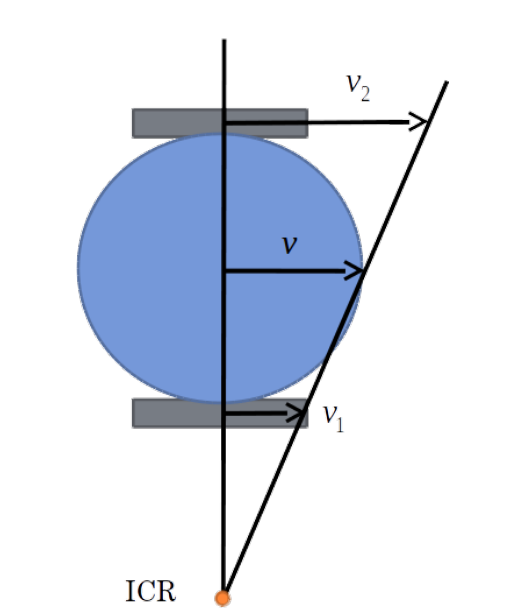
\includegraphics[scale=0.290]{img/kinematics/icr.jpeg}
\end{center}
\caption{Two wheels robot model.}
\label{icr}
\end{figure}

\begin{figure}[!htb]
\begin{center}
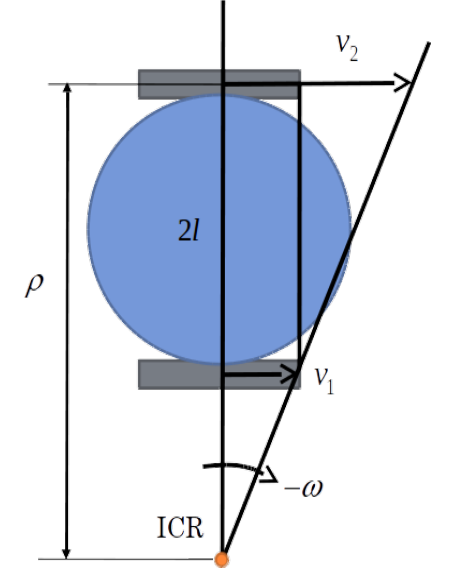
\includegraphics[scale=0.290]{img/kinematics/icr_II.jpeg}
\end{center}
\caption{Two wheels robot model.}
\label{icr_II}
\end{figure}

\section{The Longitudinal model}
\label{longitudinal_model}

In this section, we will go over the concept of the vehicle longitudinal dynamics, and the power train component models needed to generate torques on the tires. 
The longitudinal vehicle dynamic model is simply based on the dynamics of the vehicle that generate forward motion. Figure \ref{longitudinal_model_1} shows a typical vehicle longitudinal motion on an inclined road. 

\begin{figure}[!htb]
\begin{center}
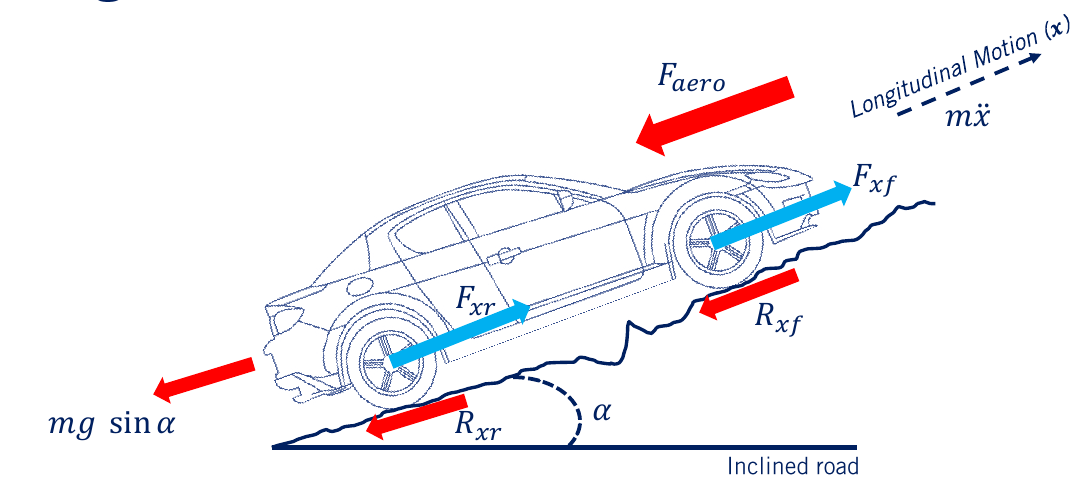
\includegraphics[scale=0.290]{img/longitudinal_model/longitudinal_model_1.jpeg}
\end{center}
\caption{Schematic of bicycle model.}
\label{longitudinal_model_1}
\end{figure}


The forces acting on the vehicle or the front and rear tire forces $F_{xf}$ and $F_{xr}$. The aerodynamic drag force $F_{aero}$ and the rolling resistance $R_{xf}$ and $R_{xr}$. 
There's also the force due to gravity, $F_g$ given by  $mg\sin(\alpha)$, where  $\alpha$ is the local road slope. 
Based on Newton's second law, the longitudinal tire forces of the front and rear tyres $F_{xf}$ and $F_{xr}$, which come from the vehicle power train must overcome the resistance forces such as the aerodynamic force $F_{aero}$, the gravitational force $f_g$, and the rolling resistance of the front and rear tires, $R_{xf}$ and $R_{xr}$. 
The imbalance between these forces defines the acceleration of the vehicle in the longitudinal direction denoted by $\ddot{X}$. 
The longitudinal dynamics equations can further be simplified by grouping the front and rear tire forces as $F_x$ and the front and rear rolling resistance forces as $R_x$. 
Further, we can assume moderate road inclinations, which means that the small angle approximation can be applied. So, that we can write

\begin{equation}
\sin(\alpha) \approx \alpha
\end{equation}

Our basic dynamic model for the longitudinal motion of a car is then as follows:

\begin{equation}
m\ddot{x} = F_{xf} + F_{xr} - f_{aero} - R_{xf} - R_{xr} - mg\sin(\alpha)
\end{equation}

 Here, $\ddot{x}$ is the inertial term that defines the vehicle's longitudinal acceleration. 
$F_x$ is the traction force generated by the power train, and $F_{aero}, R_x, F_g$, make up the total resistance forces acting on the vehicle, which we'll refer to as $F_{load}$. Note that we still need to develop models for each of the forces in this equation and define how they connect to the throttle and break inputs that our autonomous system will apply. We will do so subsequently.

\subsubsection{Aerodynamic drag}

A vehicles longitudinal motion is resisted by aerodynamic drag rolling resistance and the force due to gravity. We've already built a model for the effects of gravity, so let's move on to aerodynamics. The aerodynamic drag can typically be modeled as dependent on air density, frontal area of the vehicle, the vehicles coefficient of friction, and the current speed of the vehicle. 

\begin{equation}
F_{aero} = \frac{1}{2} C_D \rho A v^2 = C_{a} v^2
\end{equation}

Given a fixed vehicle shape and standard atmospheric pressure, we can define a simple lumped coefficient of the aerodynamic drag $C_D$, and multiply it by the velocity squared to get the drag force. 

\subsubsection{Rolling resistance}

For rolling resistance, we have a similar model which can depend on the normal force, tire pressure and characteristics, and vehicle speed. 

\begin{equation}
R_x = N(\hat{c}_{r,0} + \hat{c}_{r,1}|\dot{x}| + \hat{c}_{r,2} \dot{x}^2) \approx \hat{c}_{r,1}|\dot{x}| 
\end{equation}

If we again assume nominal operating conditions and drop the second-order terms for simplicity, we can arrive at a linear rolling resistance model, where $\hat{c}_{r,1}$ is our linear rolling resistance coefficient. In both cases, these are basic approximate models that are a good starting point for controller design. In practice, the fidelity of the model used depends on the accuracy required of the controller or the simulation environment. 


\subsubsection{Powertrain forces}

Now that we have models for the resistance forces acting on the vehicle, let's look more closely at the dry forces created by the vehicles power train. The force generated to conquer the resistance forces comes from the power train, and can be modeled as being generated by a series of components. 

\begin{figure}[!htb]
\begin{center}
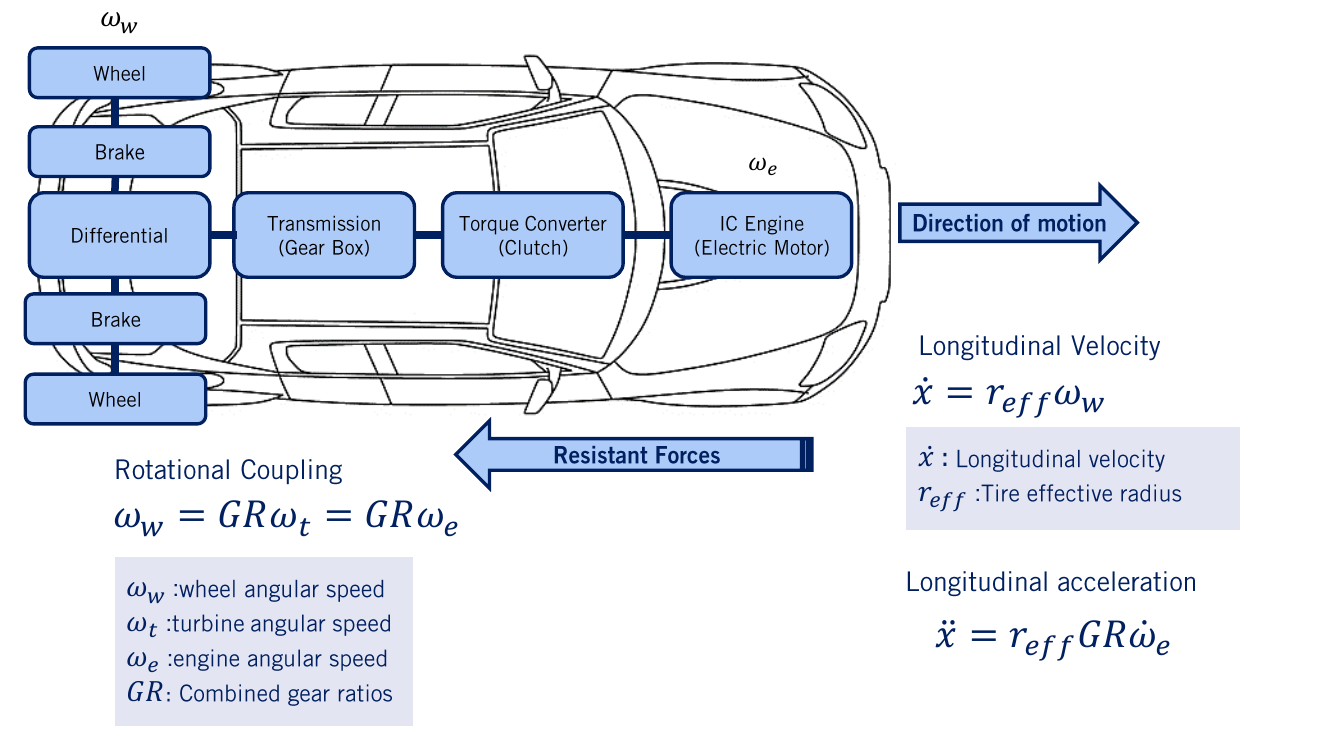
\includegraphics[scale=0.290]{img/longitudinal_model/longitudinal_model_2.jpeg}
\end{center}
\caption{Schematic of bicycle model.}
\label{longitudinal_model_2}
\end{figure}

The power generated due to the combustion in gasoline, or diesel engines, or electrochemical reactions in batteries for electric vehicles or hybrid vehicles, flow through the drive line and ultimately provide a torque to the wheels. The drive line refers to the sequence of components between the engine and the wheels, and typically includes the torque converter or clutch, the transmission or gearbox, and finally the differential. The breaks are also included in this figure, and can provide a resistance torque on the wheel hub directly. Because of the direct connection between wheel and engine when in gear, it is possible to model the relationship between the wheel speed and the engine speed as a kinematic constraint. The wheel rotation speed $\omega_w$ varies according to 
the torque converters turbine speed $\omega_t$, through several gear ratios including the torque converter, transmission, and differential. This combined gear ratio is denoted GR and changes depending on the state of the power train components. So, what gear the transmission is in, for example? 

The engine speed is equal to the turbine speed and can be used interchangeably. The vehicle forward velocity is also proportional to the 
wheel angular speed times the tire effective radius, which we will mostly model as a fixed tire radius. 
It can however be modified for higher fidelity modeling based on expected deformation of the tire due to forces and moments on the car. 
Assuming the effective tire radius, $r_{eff}$ is known, we can write that the longitudinal vehicle speed $\dot{x}$ as

\begin{equation}
\dot{x} = r_{eff}\omega_w
\end{equation}

So, if we can model the dynamics of the engine speed, we can then relate it directly to the vehicle speed through these kinematic constraints. 
This expression for velocity can be differentiated to give longitudinal acceleration in terms of the engine rotational acceleration. 
Now, let's go through the dynamic equations of each of the power train components to build a dynamic model of the overall power train. 

The wheel is the intersection between the torques coming from the power train side
and the torques acting from the external resistance forces. 
Therefore, we can present the wheel dynamics by the following first-order differential equation: 


to calculate the wheel angular speed omega w. Here T wheel is the wheel torque generated by the power train. 
We can solve for the wheel torque using this differential equation, if the tyre force $F_x$ is known, 
which can be calculated from the vehicle longitudinal dynamics derived earlier. 
The wheel torque $T$ is actually the combination of the brake torque and the output torque of the transmission 
or gearbox, as is visible on the left. 

The torque applied to the transmission is referred to as the turbine torque $T_t$ and comes from the 
torque converter which couples the engine to the transmission. 
Recall the turbine angular speed $omega_t$  of the torque converter is related to the wheel angular speed by the gear ratio GR. 
We can therefore define a similar ordinary differential equation for the turbine angular speed as our transmission dynamic model. 
Also, we can substitute in our expression for $T$ wheel from the wheel dynamics model. 
Next up is the torque converter. 
In practice, that torque converter has complex dynamics. 
When coupled, we can assume the turbine angular speed is almost the same as the engine speed. 
Therefore, we replace the turbine speed with the engine angular speed in the transmission model to form a dynamic model that includes the torque converter. 
Finally, we can define the full power train model by including the engine dynamics. 
The engine inertia term is equal to the torque produced by the engine from the combustion process 
minus the turbine torque from the torque converter, which still includes a dependence on the tire force $F_x$. 
If we return to the original longitudinal vehicle model and solve for the tire force, we see a further dependence 
on the engine rotational acceleration, which can be grouped with the terms from the engine, 
transmission, and wheel inertias. 

We now form the complete power train model and define an effective power train inertia as the sum of all the individual 
component inertias, which we'll call $J_e$. The power train model simplifies down to the following equation, 
which balances the engine torque T engine with the total load torque T load to drive the engine acceleration and thereby the vehicle longitudinal acceleration. 

\begin{itemize}
J_e \dot{\omega}_e = T_{Engine} - GR r_{eff}F_{load}
\end{itemize}

This final equation achieves what we set out to do, as it 
shows the dynamics of the whole power train system all the way from the engine to the 
external resistance forces acting on the vehicle. 

We do still need to relate the engine torque to the accelerator pedal position, 
and the brake torque to the brake pedal position. 

\section{The Bicycle model}

The previous chapter, discussed the basics of kinematic modeling and constraints and introduced the notion of the instantaneous center of rotation or ICR. 
This section, develops the kinematic bicycle model, a classic model that does surprisingly well at capturing vehicle motion in normal driving conditions. Let's get started. 


The well-known kinematic bicycle model has long been used as a suitable control-oriented model for representing vehicles because of its simplicity and adherence to the nonholonomic constraints of a car. Before we derive the model, let's define some additional variables on top of the ones we used for the two-wheeled robot. 


The bicycle model we'll develop is called the front wheel steering model, as the front wheel orientation can be controlled relative to the heading of the vehicle. 
Once again, we assume the vehicle operates on a 2D plane denoted by the inertial frame FI. 

\begin{figure}[!htb]
\begin{center}
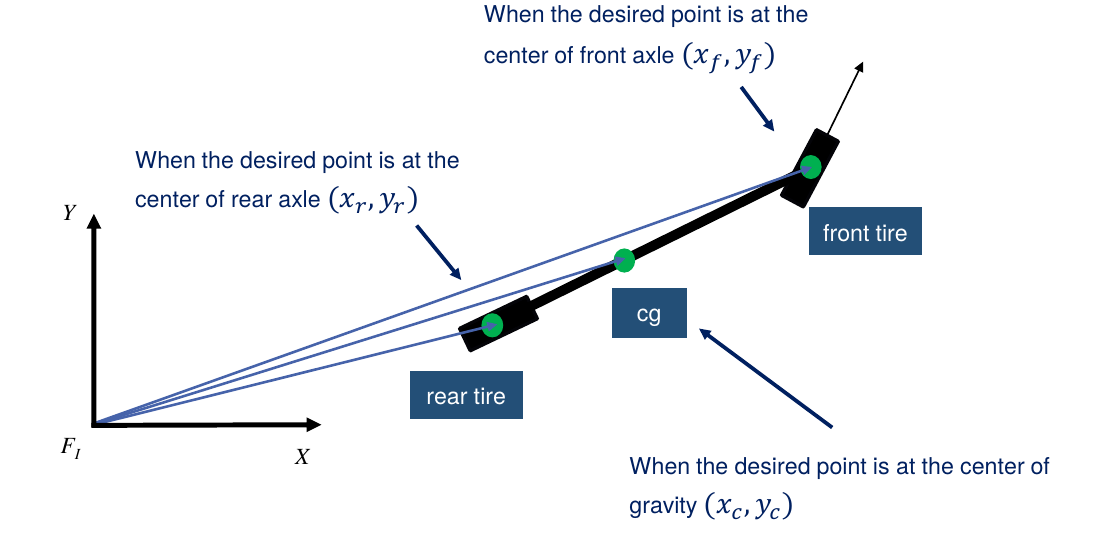
\includegraphics[scale=0.290]{img/bicycle_model/bicycle_model_1.jpeg}
\end{center}
\caption{Schematic of bicycle model.}
\label{bicycle_model_1}
\end{figure}


In the proposed bicycle model, the front wheel represents the front right and left wheels of the car, and the rear wheel represents the rear right and left wheels of the car. 
To analyze the kinematics of the bicycle model, we must select a reference point $(X, Y)$ on the vehicle which can be placed at the center of the rear axle, the center of the front axle, or at the center of gravity or CG, see figure \ref{bicycle_model_1}. 

The selection of the reference point changes the kinematic equations that result, which in turn change the controller designs that we'll use. As needed, we'll switch between reference points throughout this course. 


Let's start with the rear axle reference point model. We'll denote the location of the rear axle reference point as $x_r, y_r$ and the heading of the bicycle as $\theta$. We'll use $L$ for the length of the bicycle, measured between the two wheel axes. 

\begin{figure}[!htb]
\begin{center}
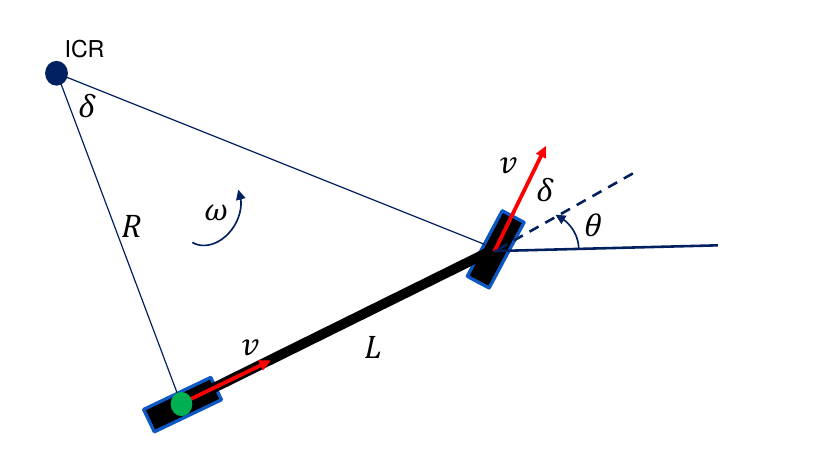
\includegraphics[scale=0.290]{img/bicycle_model/bicycle_model_2.jpeg}
\end{center}
\caption{Schematic of bicycle model.}
\label{bicycle_model_2}
\end{figure}


As with the two-wheeled robot, these are our main model states. The inputs for the bicycle model are slightly different than those for the two-wheeled robot, as we now need to define a steering angle $\delta$ for the front wheel. This angle and is measured relative to the forward direction of the bicycle. The velocity is denoted $v$ and points in the same direction as each wheel. 
This is an assumption referred to as the no slip condition, which requires that our wheel cannot move laterally or slip longitudinally either. 
It is the same assumption that allows us to compute the forward speed of the two-wheeled robot based on the rotation rates of its wheels, see figure \ref{bicycle_model_2}. 
Because of the no slip condition, we once again have that $\omega$, the rotation rate of the bicycle, is given by

\begin{equation}
\dot{\theta} = \omega = \frac{v}{r}
\end{equation}


From the similar triangles formed by $L$ and $R$, and $v$ and $\delta$, we see that:

\begin{equation}
\tan(\delta) = \frac{L}{R}
\end{equation}


By combining both equations, we can find the relation between the rotation rate of the vehicle $\omega$, and the steering angle $\delta$:
\begin{equation}
\omega = \frac{v\tan(\delta)}{L}
\end{equation}

We can now form the complete kinematic bicycle model for the rear axle reference point. 
\begin{figure}[!htb]
\begin{center}
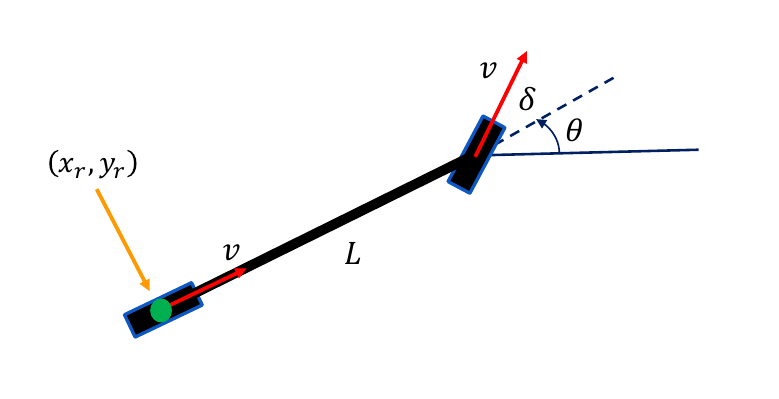
\includegraphics[scale=0.290]{img/bicycle_model/bicycle_model_3.jpeg}
\end{center}
\caption{Schematic of bicycle model with rear axle reference point.}
\label{bicycle_model_3}
\end{figure}
Based on this model configuration, the complete bicycle model with respect to the  reference point in the $x$ and $y$ direction is given by:
\begin{eqnarray}
\dot{x}_r = v\cos(\theta) \\
\dot{y}_r = v\sin(\theta) \\
\dot{\theta} = \frac{v\tan(\delta)}{L}
\end{eqnarray}


The bicycle kinematic model can be reformulated when the center of the front axle is taken as the reference point $x, y$ as sbhown in figure. 

\begin{figure}[!htb]
\begin{center}
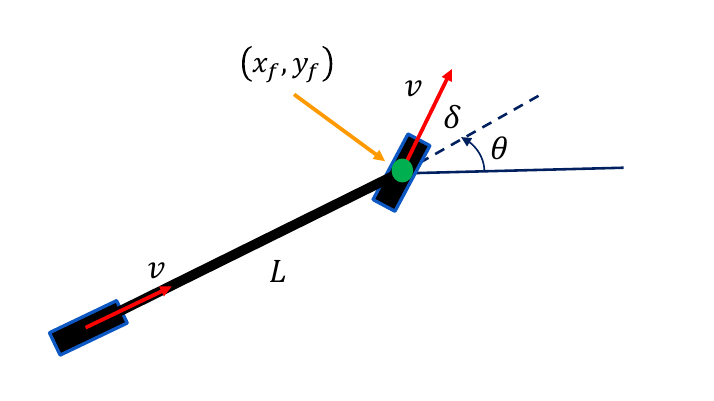
\includegraphics[scale=0.290]{img/bicycle_model/bicycle_model_4.jpeg}
\end{center}
\caption{Schematic of bicycle model with front axle reference point.}
\label{bicycle_model_4}
\end{figure}


The velocity points in the direction of the front wheel this time, which is defined by the summation of $\delta$ and $\theta$. Working through the derivation leads to the following kinematic model for the vehicle. 

\begin{eqnarray}
\dot{x}_f = v\cos(\theta + \delta) \\
\dot{y}_f = v\sin(\theta + \delta) \\
\dot{\theta} = \frac{v\sin(\delta)}{L}
\end{eqnarray}

The last scenario is when the desired point is placed at the center of gravity or center of mass as shown in figure \ref{bicycle_model_5}. 



\begin{figure}[!htb]
\begin{center}
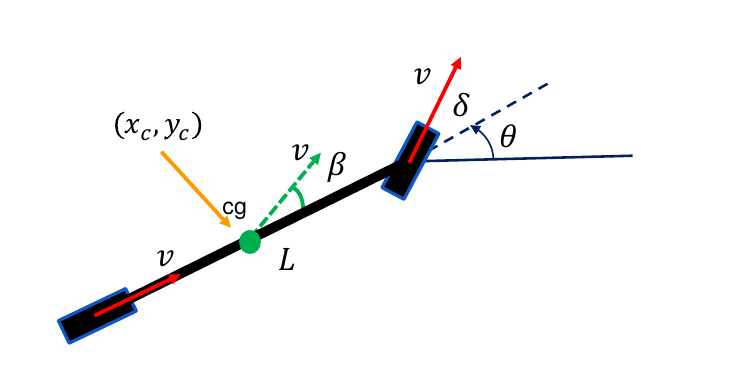
\includegraphics[scale=0.290]{img/bicycle_model/bicycle_model_5.jpeg}
\end{center}
\caption{Schematic of bicycle model with front axle reference point.}
\label{bicycle_model_5}
\end{figure}

Because of the no slip constraints we enforce on the front and rear wheels, the direction of motion at the CG is slightly different from the forward velocity direction in either wheel and from the heading of the bicycle. This difference is called the slip angle or side slip angle, which we'll refer to as $\beta$, and is measured as the angular difference between the velocity at the CG and the heading of the bicycle. This definition of side slip angle will also apply when we move to dynamic modeling of vehicles, where it can become more pronounced. The kinematic model with the reference point at the $CG$ can be derived similarly to both the rear and forward axle reference point models. We end up with the following formulation, which we'll use as the basis for our modeling of the dynamics of vehicles as well. 

\begin{eqnarray}
\dot{x}_c = v\cos(\theta + \beta) \\
\dot{y}_f = v\sin(\theta + \beta) \\
\dot{\theta} = \frac{v\cos(\beta)\tan(\delta)}{L} \\
\end{eqnarray}


Lastly, because of the no slip condition, we can compute the slip angle from the geometry of our bicycle model. Given $LR$, the distance from the rear wheel to the CG, the slip angle $\beta$ is equal to:

\begin{equation}
\beta = arctan(\frac{l_r \tan(\delta)}{L})
\end{equation}

Finally, it is not usually possible to instantaneously change the steering angle of a vehicle from one extreme of its range to another, as is currently possible with our kinematic model. Since $\delta$ is an input that would be selected by a controller, there is no restriction on how quickly it can change which is somewhat unrealistic. Instead, our kinematic models can be formulated with four states: $x, y, \theta$, and the steering angle $\delta$. 
If we assume we can only control the rate of change of the steering angle $\phi$, we can simply extend our model to include $\delta$ as a state and use the steering rate $\phi$ as our modified input. 

Our kinematic bicycle model is now complete.  Our kinematic bicycle model takes as inputs the velocity and the steering rate $\phi$. The state of the system, including the positions $x_c, y_c,$ the orientation $\theta$, and the steering angle $\delta$, evolve according to our kinematic equations from the model, which satisfy the no slip condition. We can now use this model to design kinematic steering controllers. 


\section{Questions}
\label{questions_vehicle_kinematics_and_dynamics}



